\documentclass[notitlepage,a4paper,10pt,twoside]{article}

%\usepackage{mathpazo} 
\usepackage{ngerman} 
\usepackage[latin1]{inputenc} 
\usepackage[T1]{fontenc} 
\usepackage[pdftex]{graphicx} 
\usepackage[pdftex,bookmarks=true,colorlinks,linkcolor=blue,urlcolor=blue,citecolor=blue]{hyperref}

\sloppy

%opening
\title{Daten verschl�sseln}
\author{mit DM-Crypt f�r Linux}
\date{\today}

\hypersetup {
    pdftitle= { Daten verschl�sseln mit DM-Crypt f�r Linux }
    pdfkeywords= {Daten verschl�sseln Verschl�sselung DM-Crypt Linux cryptsetup }
}


\begin{document}
\maketitle
\tableofcontents

\section{Einleitung}
Dass die Verschl�sselung von Daten der Erhaltung einer Privatsph�re dient, bemerkt man sp�testens, wenn ein USB-Stick verloren geht. Wird ein Laptop gestohlen, m�chte man die Fotosammlung sicher nicht im Internet sehen.\\

Investigative Journalisten, Rechtsanw�lte und auch Priester haben das Recht und die Pflicht, ihre Informanten bzw. Klienten zu sch�tzen. Sie sollten sich fr�hzeitig Gedanken �ber ein Konzept zur Verschl�sselung machen. Es ist wirklich �rgerlich, wenn die Rote Hilfe einen unverschl�sselten Datentr�ger mit Mitgliederdaten verliert. Das kann ernste Konsequenzen haben.\\

Als Whistleblower sind besondere Anforderungen an die Datensicherheit zu stellen. Neben der sicheren Aufbewahrung kommt es auch darauf an, keine Spuren auf den Rechnern zu hinterlassen. Im Fall Bradley Mannings konnten Forensiker viele Daten wieder herstellen

Die kurzen Beispiele zeigen, dass unterschiedliche Anforderungen an eine Verschl�sselung bestehen k�nnen. Bevor man wild anf�ngt, alles irgendwie zu verschl�sseln, sollte man sich Gedanken �ber die Bedrohung machen, gegen die man sich sch�tzen will:
\begin{enumerate}
 \item \textbf{Schutz sensibler Daten} wie z.B. Passwortlisten, Revocation Certificates o.�. erfordert die Speicherung in einem Container oder verschl�sselten Archiv, welches auch im normalen Betrieb geschlossen ist.
\item \textbf{Schutz aller pers�nlichen Daten} bei Verlust oder Diebstahl von Laptop oder USB-Stick erfordert eine Software, die transparent arbeitet ohne den Nutzer zu behindern und bei korrekter Anmeldung m�glichst automatisch den Daten-Container �ffnet (beispielsweise TrueCrypt f�r WINDOWS oder DM-Crypt f�r Linux). 
\item \textbf{Backups auf externen Medien} enthalten in der Regel die wichtigen privaten Daten und sollten ebenfalls verschl�sselt sein. Dabei sollte die Wiederherstellung auch bei totalem Datenverlust m�glich sein. Es ist nicht sinnvoll, die Daten mit einem PGP-Schl�ssel zu chiffrieren, der nach einem Crash nicht mehr verf�gbar ist.
\item Wer eine \textbf{Manipulation der Sytemdaten} bef�rchtet, kann seinen Rechner komplett verschl�sseln (mit Truecrypt f�r WINDOWS, DM-Crypt f�r Linux oder GELI f�r FreeBSD).\\
\end{enumerate}

Zur \textbf{Herausgabe von Schl�sseln} im Fall einer Beschlagnahme des Rechners oder verschl�sselten Datentr�gers gibt es immer wieder Missverst�ndnisse.\\

In Deutschland gelten folgende gesetzlichen Reglungen:
\begin{itemize}
 \item Richten sich die Ermittlungen gegen den Besitzer des Rechners oder Datentr�gers muss man grunds�tzlich keine Keys herausgeben.
\item Richten sich die Ermittlungen gegen Dritte, kann man die Herausgabe von Keys verweigern, wenn man sich auf das Recht zur Zeugnisverweigerung berufen oder glaubhaft(!) versichern kann, dass man sich damit selbst belasten w�rde. Im Zweifel sollte man einen Anwalt konsultieren.
\end{itemize}

In Gro�britannien ist es bereits anders. Gem�� dem dort seit Oktober 2007 geltendem RIPA-Act k�nnen Nutzer von Verschl�sselung unter Strafandrohung zur Herausgabe der Schl�ssel gezwungen werden. Es drohen bis zu 2 Jahre Gef�ngnis oder Geldstrafen. Das die Anwendung des Gesetzes nicht auf die b�sen Terroristen beschr�nkt ist, kann man bei Heise.de nachlesen. Es wurde als ersten gegen eine Gruppe von Tiersch�tzern angewendet.\footnote{ \href{http://www.heise.de/newsticker/meldung/99313}{http://www.heise.de/newsticker/meldung/99313}}\\

Bei Einreise in die USA sind die Grenzbeh�rden berechtigt, elektronische Ger�te (Laptops und Smartphones) zu durchsuchen. Eine Herausgabe von Passw�rtern kann ohne Durchsuchungs�beschluss nicht erzwungen werden, aber die Beh�rden k�nnen das Ger�t aber zur weiteren Untersuchung einziehen, wenn man das Passwort nicht heraus geben will. Die EFF.org r�t, mit einer leeren, unverschl�sselten Festplatte einzureisen und ein datenloses Handy zu nutzen: \href{https://www.eff.org/wp/defending-privacy-us-border-guide-travelers-carrying-digital-devices}{https://www.eff.org/wp/defending-privacy-us-border-guide-travelers-carrying-digital-devices}

\subsubsection*{Das Container-Konzept}
Der Container ist eine passende Metapher f�r das Konzept der vorgestellten Tools \textit{Truecrypt} und \textit{DM-Crypt}. Ein Container steht rum und nimmt Platz weg, egal ob er leer oder voll ist. In diesem Fall belegt der Container Platz auf der Festplatte oder dem USB-Stick.\\

Ist der Container verschlossen, kommt niemand an die dort lagernden Daten heran. Mit einem Schl�ssel kann der Container ge�ffnet werden (gemounted: in das Dateisystem eingef�gt) und jeder, der an einem offenen Container vorbeikommt, hat Zugriff auf die dort lagernden Daten. Als Schl�ssel dient eine Passphrase und/oder Schl�sseldatei(en).\\

Der Zugriff auf Dateien innerhalb des ge�ffneten Containers erfolgt mit den Standardfunktionen f�r das �ffnen, Schlie�en und L�schen von Dateien. Auch Verzeichnisse k�nnen angelegt bzw. gel�scht werden. Die Verschl�sselung erfolgt transparent ohne weiteres Zutun des Nutzers.\\

Ein Container sch�tzt die Daten nur, wenn er geschlossen ist! Wenn man keinen ZUgriff auf die Daten braucht, sollte man den Container schlie�en. Einerseits ist bei einem ge�ffneten Container ein direkter Zugriff auf die Daten m�glich. Au�erdem k�nnen bei einem ge�ffneten Container die kryptografischen Schl�ssel aus dem RAM des Rechners ausgelesen und sp�ter zum Entschl�sseln der Daten genutzt werden. Elcomsoft bietet mit dem \textit{Forensic Disk Decryptor} eine Tool f�r diesen Angriff auf Truecrypt, PGP und Bitlocker.\footnote{ \href{http://www.elcomsoft.com/news/531.html}{http://www.elcomsoft.com/news/531.html}}
\newpage
\section{DM-Crypt f�r Linux}
DM-Crypt ist seit Version 2.6.4 fester Bestandteil des Linux-Kernels und somit in allen aktuellen Distributionen enthalten. Es nutzt den Device-Mapper. Folgende Software wird au�erdem ben�tigt:\\

\begin{itemize}
 \item Das Tool \textbf{cryptsetup} (mit LUKS-Support) kann zum Erstellen, �ffnen und Schlie�en der verschl�sselten Container eingesetzt werden. Aktuelle Distributionen enthalten es: Debian GNU/Linux im Packet \textit{cryptsetup}, SuSE-Linux im Packet \textit{util-linux-crypto}.\\

Einige Distributionen installieren das Tool unter dem Namen \textit{cryptsetup-luks}. Die im Folgenden beschrieben Befehlen sind dann entsprechend anzupassen. Besser w�re es, einen Link zu erstellen. Dann funktionieren auch die Scripte \textit{mount.crypt} und \textit{umount.crypt} aus der Sammlung pam-mount.
\begin{verbatim}
  # ln -s /usr/sbin/cryptsetup-luks /sbin/cryptsetup
\end{verbatim} 

\item Das Packet \textbf{pmount} enth�lt einen Wrapper f�r das \textit{mount}-Kommando, welcher automatisch verschl�sselte Laufwerke erkennt und vor dem Einbinden das Passwort abfragt. Aktuelle Debian-Distributionen verwenden es standardm��ig.

\item Die Sammlung \textbf{pam-mount} enth�lt weitere Scripte, das das �ffnen und Schlie�en verschl�sselter Container vereinfachen. Die Scripte erm�glichen beispielsweise des �ffnen eines Containers automatisch beim Login. Unter Debian installiert man die Tools wie �blich mit
\begin{verbatim}
   # aptitude install libpam-mount.
\end{verbatim}

\item Das Kernelmodul \textbf{dm\_crypt} muss vor der Verwendung der oben genannten Scripte geladen werden. In Abh�ngigheit von der bevorzugten Distribution und der Installationsvariante wird das Modul bereits beim Booten geladen oder ist statisch in \textit{initrd.img} eingebunden. Einfach probieren.\\

Sollte beim Erstellen oder �ffnen eines verschl�sselten Containers die folgende Fehlermeldung auftreten:
\begin{verbatim}
Command failed: Failed to setup dm-crypt key mapping.
Check kernel for support for the aes-cbc-essiv:sha256 cipher
\end{verbatim}

ist das Kernel-Modul \textit{dm\_crypt} zu laden:
\begin{verbatim}
   # modprobe dm_crypt
\end{verbatim}

Au�erdem sollte das Modul in die Liste der beim Systemstart zu ladenen Module eingef�gt werden. In der Datei \textit{/etc/modules} ist die Zeile \textit{dm\_crypt} anzuh�ngen.
\end{itemize}
 
\subsection{Gedanken zum Passwort}
An Stelle von \textit{Passwort} sollte man vielleicht die Bezeichnung \textit{Passphrase} bevorzugen. Sie suggeriert, dass es auch ein wenig l�nger sein darf und dass Leerzeichen durchaus erlaubt sind.\\

Eine gute Passphrase sollte leicht merkbar aber schwer zu erraten sein. Au�er Buchstaben sollte sie auch Zahlen und Sonderzeichen enthalten und etwa 20 Zeichen lang sein. Soetwas sch�ttelt man nicht einfach aus dem �rmel. Wie w�re es mit folgender Phrase:

\begin{center}
\texttt{ das geht nur \%mich\% \_AN\_}
\end{center}

Zus�tzlich zur Passphrase k�nnen auch Keyfiles als Schl�ssel genutzt werden. Damit ist es m�glich, eine Zwei-Faktor-Authentifizierung aufzubauen: eine Passphrase, die man im Kopf hat, und ein Keyfile, welches man in der Hand hat. Ein Angreifer m�sste beides erlangen.\\

Die LUKS-Erweiterung von \textit{cryptsetup} erlaubt es, bis zu 8 Passphrasen und Keyfiles zum �ffnen eines Containers zu nutzen. Damit ist es m�glich, mehreren Nutzern den Zugriff mit einem eigenen Passwort zu erlauben.\\

Soll ein verschl�sselter Container mit dem Login eines Nutzers automatisch ge�ffnet werden, muss eines der 8 m�glichen Passw�rter mit dem Login-Passwort des Nutzers identisch sein. Login-Manager wie KDM oder GDM k�nnen das eingegebene Passwort an das pam-mount Modul weiterreichen. Dieses Feature kann beispielsweise f�r ein verschl�sseltes \textit{/home} Verzeichnis genutzt werden.\\

WICHTIG: bei �nderung des Login-Passwortes muss auch das Paswort f�r den Container ge�ndert werden. Sie werden nicht automatisch synchronisiert.

\subsection{Verschl�sselten Container erstellen}
Alle folgenden Schritte sind als \textit{root} auszuf�hren. Zum Aufw�rmen soll zuerst die Partition \textit{/dev/hda4} verschl�sselt werden. Debian und Ubuntu enthalten das Skript <em>luksformat</em>, dass alle Aufgaben erledigt.  

\begin{verbatim}
   # luksformat -t ext3 /dev/hda4
\end{verbatim}

Das ist alles. Der Vorgang dauert ein wenig und es wird 3x die Passphrase abgefragt. Ein Keyfile kann dieses Script nicht nutzen! Um einen USB-Stick komplett zu verschl�sseln, w�hlt man \textit{/dev/sdb1} oder \textit{/dev/sda1}. Es ist vor(!) Aufruf des Kommandos zu pr�fen, unter welchem Device der Stick zur Verf�gung steht.\\

\subsubsection*{Verschl�sselten Container erstellen f�r Genie�er}

Am Beispiel einer verschl�sselten Containerdatei werden die einzelnen Schritte beschrieben, welche das Script \textit{luksformat} aufruft. Soll eine Partition (Festplatte oder USB-Stick) verschl�sselt werden, entfallen die Schritte 1 und 8. Das als Beispiel genutzte Device \textit{/dev/loop5} ist durch die Partition zu ersetzen, beispielsweise \textit{/dev/hda5} oder \textit{/dev/sdb1}. 

\begin{enumerate}
 \item Zuerst ist eine leere Imagedatei zu erstellen. Im Beispiel wird es unter dem Dateinamen \textit{geheim.luks} im aktuellen Verzeichnis erstellt. Der Parameter \textit{count} legt die Gr��e in MByte fest. Anschlie�end ist das Image als Loop-Device einzubinden. Das Kommando \textit{losetup -f} ermittelt das n�chste freie Loop-Device (Ergebnis: \textit{loop0}).
\begin{verbatim}
   # dd if=/dev/zero of=geheim.luks bs=1M count=100
   # losetup -f
   /dev/loop0
   # losetup /dev/loop0 geheim.luks
\end{verbatim} 
\item Die ersten 2 MByte sind mit Zufallswerten zu f�llen. Das F�llen der gesamten Datei w�rde sehr lange dauern und ist nicht n�tig:
\begin{verbatim}
   # dd if=/dev/urandom of=/dev/loop0 bs=1M count=2
\end{verbatim}
\item Anschlie�end erfolgt die LUKS-Formatierung mit der Festlegung der Verschl�sselung. Die Option -y veranla�t eine doppelte Abfrage des Passwortes, das \textit{keyfile} ist optional
\begin{verbatim}
   # cryptsetup luksFormat -c aes-cbc-essiv:sha256 -s 256 -y 
                         /dev/loop0 [ keyfile ]
\end{verbatim}

\item Das formatierte Device wird dem Device-Mapper unterstellt. Dabei wird das zuvor eingegebene Passwort abgefragt. Das Keyfile ist nur anzugeben, wenn es auch im vorherigen Schritt verwendet wurde. Der <name> kann frei gew�hlt werden. Unter /dev/mapper/<name> wird sp�ter auf den verschl�sselten Container zugegriffen:
\begin{verbatim}
   # cryptsetup luksOpen /dev/loop0 <name> [ keyfile ]
\end{verbatim}
\item Wer paranoid ist, kann das verschl�sselte Volume mit Zufallszahlen f�llen. Der Vorgang kann in Abh�ngigkeit von der Gr��e der Containerdatei sehr lange dauern:
\begin{verbatim}
   # dd if=/dev/urandom of=/dev/mapper/<name>
\end{verbatim}
\item Ein Dateisystem wird auf dem Volume angelegt:
\begin{verbatim}
   # mkfs.ext3 /dev/mapper/<name>
\end{verbatim}
\item Das Volume ist nun vorbereitet und wird wieder geschlossen:
\begin{verbatim}
   # cryptsetup luksClose <name>
\end{verbatim}
\item Die Containerdatei wird ausgeh�ngt:
\begin{verbatim}
   # losetup -d /dev/loop0
\end{verbatim} 
\end{enumerate}

\subsection{Passw�rter verwalten}
Mit root-Rechten ist es m�glich, bis zu 7 zus�tzliche Passw�rter f�r das �ffnen eines Containers festzulegen oder einzelne Passw�rter wieder zu l�schen.\\

F�r das Hinzuf�gen eines Passwortes zu der verschl�sselten Imagedatei \textit{geheim.img} im aktuellen Verzeichnis ist diese zuerst einzuh�ngen, beispielsweise als \textit{/dev/loop5}. Dieser Schritt entf�llt f�r Partitionen:
\begin{verbatim}
   # losetup /dev/loop5 geheim.luks
\end{verbatim}

Das Hinzuf�gen eines Passwortes und damit eines neuen Keyslots erfolgt mit folgendem Kommando, wobei als <device> beispielsweise \textit{/dev/loop5} f�r die eingebundene Imagedatei oder \textit{/dev/hda5} f�r eine Festplattenpartition anzugeben ist. Das Keyfile ist optional.
\begin{verbatim}
   # cryptsetup luksAddKey <device> [ keyfile ]
\end{verbatim} 

Ein Keyslot und das zugeh�rige Passwort k�nnen mit folgendem Kommando wieder entfernt werden:
\begin{verbatim}
   # cryptsetup luksKillSlot <device> <slot>
\end{verbatim}

Als <slot> ist die Nummer des Keyslots anzugeben, eine Zahl von 0 is7. Es ist also n�tig, sich zu merken, welches Passwort auf welchen Keyslot gelegt wurde. Eine �bersicht, welche Keyslots belegt und welche noch frei sind, liefert \textit{luksDump}:
\begin{verbatim}
   # cryptsetup luksDump <device>
   LUKS header information for <device>
   ...
   Key Slot 0: DISABLED
   Key Slot 1: ENABLED
        Iterations:
        Salt:

        Key material offset:
        AF stripes:
   Key Slot 2: DISABLED
   Key Slot 3: DISABLED
   Key Slot 4: DISABLED
   Key Slot 5: DISABLED
   Key Slot 6: DISABLED
   Key Slot 7: DISABLED
\end{verbatim}

\subsection{Verschl�sselten Container �ffnen/schlie�en}
Aktuelle Distributionen wie Debian oder Ubuntu erkennen verschl�sselte Partitionen auf Festplatten und USB-Sticks automatisch und fragen die Passphrase ab, sobald das Ger�t erkannt wird. Einfach Anschlie�en, auf den Passwort-Dialog wie im Bild \ref{abb:dmcrypt_open} warten - fertig.

\begin{figure}[htb]
\begin{center}
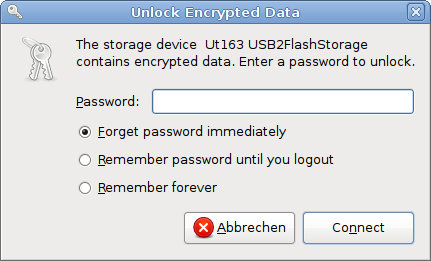
\includegraphics[scale=0.55]{../screenshots/Unlock_Encrypted_Data.png}
\caption{Passwort-Abfrage f�r verschl�sselten USB-Stick}
\label{abb:dmcrypt_open}
\end{center}
\end{figure}

\subsubsection*{Auf der Kommandozeile}
Sollte es mit dem automatischem �ffnen des verschl�sselten USB-Sticks nicht funktionieren, kann man auf der Kommandozeile nachhelfen. \textit{pmount} arbeitet mit User-Privilegien und bindet die Partition unter \textit{/media} ein. pmount kann keine Containerdateien �ffnen.
\begin{verbatim}
   > pmount /dev/sda1 
   Enter LUKS passphrase:
\end{verbatim}

Geschlossen wird der Container mit \textit{pumount}:
\begin{verbatim}
   > pumount /dev/sda1 
\end{verbatim}

Die Sammlung pam-mount enth�lt zwei weitere Scripte, welche die Arbeit mit verschl�sselten Containerdateien vereinfachen. Wurde au�erdem \textit{sudo} entsprechend konfiguriert, stehen die folgenden Kommandos jedem Nutzer zur Verf�gung. Eine verschl�sselte Partition (beispielsweise der USB-Stick unter /dev/sda1) kann mit folgendem Kommando ge�ffnet und im Verzeichnis /mnt eingebunden werden:
\begin{verbatim}
   > sudo /sbin/mount.crypt /dev/sda1 /mnt
   Enter LUKS passphrase:
\end{verbatim}

Das folgende Kommando �ffnet die verschl�sselte Imagedatei \textit{geheim.luks} aus dem aktuellen Verzeichnis und h�ngt sie unter \textit{/mnt} in das Dateisystem ein:
\begin{verbatim}
   > sudo /sbin/mount.crypt  geheim.luks  /mnt  -o  loop
   Enter LUKS passphrase:
\end{verbatim}

Geschlossen wird der Container mit folgendem Komando:

\begin{verbatim}
   > sudo /sbin/umount.crypt /mnt
\end{verbatim}

F�r h�ufig genutzte Container k�nnte man einen Men�eintrag oder ein Desktop-Icon anlegen. Dabei ist zu beachten, dass die Option \textit{Im Terminal ausf�hren} aktiviert wird! Anderenfalls kann man keine Passphrase eingeben.

\subsubsection*{F�r jene, die es genau wissen wollen}
Das �ffnen einer Containerdatei auf der Komadozeile erfordert drei Schritte als \textit{root}. Als erstes ist die verschl�sselte Imagedatei einzuh�ngen. Dieser Schritt entf�llt f�r Partitionen. Im zweiten Schritt ist das verschl�sselte Device dem Device-Mapper zu unterstellen. Der Name kann dabei frei gew�hlt werden. Im dritten Schritt kann es mit \textit{mount} in das Dateisystem eingeh�ngt werden, beispielsweise nach \textit{/mnt}.
\begin{verbatim}
   # losetup  /dev/loop5  geheim.luks
   # cryptsetup  luksOpen  /dev/loop5  <name> [ keyfile ]
   # mount  /dev/mapper/<name>  /mnt
\end{verbatim}

Das Schlie�en des Containers erfolgt in umgekehrter Reihenfolge:
\begin{verbatim}
   # umount  /mnt
   # cryptsetup  luksClose  <name>
   # losetup -d /dev/loop5
\end{verbatim}

\subsubsection*{Komfortabel beim Login}
Mit Hilfe des Modules pam-mount ist es m�glich, das Anmeldepasswort zu nutzen, um standardm��ig beim Login einen oder mehrere Container zu �ffnen. Insbesondere f�r verschl�sselte /home Partitionen ist dies sinnvoll und komfortabel.\\

Folgende Konfigurationen sind f�r einen Crypto-Login anzupassen:
\begin{enumerate}
 \item \textbf{PAM-Konfiguration:} Dem PAM-D�mon ist mitzuteilen, dass er das Modul \textit{mount} zu verwenden hat und das Login-Passwort zu �bergeben ist. Gut vorbereitete Distributionen wie Debian und aktuelle Ubuntu(s) ben�tigen nur einen Eintrag in den Dateien \textit{/etc/pam.d/login}, \textit{/etc/pam.d/kdm} und \textit{/etc/pam.d/gdm}:
\begin{verbatim}
   @include common-pammount
\end{verbatim}

\item \textbf{pam-mount Modul:} Das Modul wird konfiguriert in der XML-Datei \textit{/etc/security/pam\_mount.conf.xml}. Am Anfang der Datei findet man eine Section f�r Volumes, die beim Login ge�ffnet werden sollen. Im ersten Beispiel wird bei allen Logins die verschl�sselte Partition /dev/hda4 als /home eingebunden:
\begin{verbatim}
<volume fstype="crypt" path="/dev/hda4" mountpoint="/home" />
\end{verbatim}

Das zweite Beispiel zeigt die Einbindung einer verschl�sselten Containerdatei /geheim.luks als HOME f�r den User pitschie. Die Containerdatei wird nur ge�ffnet, wenn Pitschie sich anmeldet.
\begin{verbatim}
<volume user="pitschie" fstype="crypt" path="/geheim.luks" 
        mountpoint="/home/pitschie" options="loop" />
\end{verbatim}


\item \textbf{fstab:} Da beim Booten keine Partition nach \textit{/home} gemountet werden soll, ist evtl. der entsprechende Eintrag in der Datei \textit{/etc/fstab} zu l�schen.
\end{enumerate}

\subsection{Debian GNU/Linux komplett verschl�sseln}
In einem komplett verschl�sselten Sytem sind sowohl die Daten als auch die Systemkonfiguration und Software verschl�sselt. Debian ab Version 4.0r1 (etch) bietet bereits beim Installieren die Option, ein komplett verschl�ssltes System unter Ausnutzung der gesamten Festplatte zu installieren. Lediglich f�r \textit{/boot} bleibt ein kleiner unverschl�sselter Bereich.\\

Um diese einfache Variante zu nutzen, w�hlt man im Installations-Dialog \textit{Festplatte partitionieren} die Option \textit{Gef�hrt - gesamte Platte mit verschl�sseltem LVM}. Im folgenden Schritt ist die Passphrase einzugeben, welche das System sichert. Diese Passphrase wird sp�ter bei jedem Bootvorgang abgefragt.
\begin{verbatim}
 Partitionsmethode:

    Gef�hrt - verwende vollst�ndige Festplatte
    Gef�hrt - gesamte Platte verwenden und LVM einrichten
  > Gef�hrt - gesamte Platte mit verschl�sseltem LVM 
    Manuell 
\end{verbatim} 

Ubuntu-Nutzer k�nnen die \textbf{alternate desktop cd} nutzen, die kein Live-System enth�lt, daf�r aber mehr Optionen f�r die Installation bietet. Die Standard-Edition von Ubuntu bietet dieses Feature nicht!\\

Ein vollst�ndig verschl�sseltes System macht es b�swilligen Buben sehr schwer, bei einem \textit{heimlichen Hausbesuch} die Software zu manipulieren und einen Trojaner zu installieren. Es ist jedoch nicht unm�glich. Wer noch einen Schritt weiter gehen will, erstellt nach der Installation eine bootf�hige CD-ROM mit einer Kopie des sauberen Verzeichnis \textit{/boot} und bootet in Zukunft immer von der CD. (Oder man geht zum Psychater und l�sst seine Paranoia behandeln.)\\

Man sollte nicht aus Zeitgr�nden auf ein �berschreiben der alten Daten mit Zufallszahlen verzichten. Um die Position verschl�sselter Daten auf der Platte zu verstecken und Daten der alten Installation zu vernichten, bietet die Installationsroutine die Option, den Datentr�ger mit Zufallszahlen zu �berschreiben. Das dauert zwar einige Zeit, ist aber ein sinnvolles Feature.\\

\subsection{HOME-Verzeichnis verschl�sseln}
Die Verschl�sselung der pers�nlichen Daten im \$HOME-Verzeichnis bieten alle Linux-Distributionen bei der Installation an. Wer keine Komplettverschl�sselung nutzen m�chte, sollte zumindest diese Option aktivieren. Der Container mit den verschl�sselten Daten wird beim Login automatisch ge�ffnet. Die Nutzung ist vollst�ndig transparent. Bei Verlust des Laptops sind die Daten jedoch gesch�tzt.

\subsection{SWAP und /tmp verschl�sseln}
Das \textit{/tmp}-Verzeichnis und der SWAP Bereich k�nnen unter Umst�nden pers�nliche Informationen enthalten, die im Verlauf der Arbeit ausgelagert wurden. Wenn eine komplette Verschl�sselung des Systems nicht m�glich ist, sollte man verhindern, das lesbare Datenr�ckst�nde in diesen Bereichen verbleiben.\\

Das Verzeichnis \textit{/tmp} kann man im RAM des Rechners ablegen, wenn dieser hinreichend gro� dimensioniert ist. Mit dem Ausschalten des Rechners sind alle Daten verloren. Um diese Variante zu realisieren bootet man den Rechner im abgesicherten Mode, beendet die grafische Oberfl�che (X-Server) und l�scht alle Dateien in \textit{/tmp}. In der Datei \textit{/etc/fstab} wird folgender Eintrag erg�nzt:
\begin{verbatim}
    tmpfs  /tmp  tmpfs    defaults,size=256m   0 0
\end{verbatim}

Die Bereiche SWAP und \textit{/tmp} k�nnen im Bootprozess als verschl�sselte Partitionen mit einem zuf�lligen Passwort initialisiert und eingebunden werden. Mit dem Ausschalten des Rechners ist das Passwort verloren und ein Zugriff auf diese Daten nicht mehr m�glich.\\

\textbf{Achtung:} Suspend-to-RAM und Suspend-to-Disk funtionieren mit einer verschl�sselten SWAP-Partition noch nicht.

\subsubsection*{Debian GNU/Linux}
Debian und Ubuntu enthalten ein Init-Script, welches eine einfache Verschl�sselung von SWAP und \textit{/tmp} erm�glicht, wenn diese auf einer eigenen Partition liegen.\\

In der Datei \textit{/etc/crypttab} sind die folgenden Zeilen einzuf�gen, wobei \textit{/dev/hda5} und \textit{/dev/hda8} durch die jeweils genutzten Partitionen zu ersetzen sind:

\begin{verse}
cryptswp\hspace{1cm}/dev/hda5\hspace{1cm}/dev/urandom\hspace{1cm}swap\\
crypttmp\hspace{1cm}/dev/hda8\hspace{1cm}/dev/urandom\hspace{1cm}tmp
\end{verse}

In der Datei \textit{/etc/fstab} sind die Eintr�ge f�r swap und /tmp anzupassen:

\begin{verse}
/dev/mapper/cryptswp\hspace{0.5cm}none\hspace{0.5cm}swap\hspace{0.5cm}sw\hspace{0.5cm}0 0\\
/dev/mapper/crypttmp\hspace{0.5cm}/tmp\hspace{0.5cm}ext2\hspace{0.5cm}defaults\hspace{0.5cm}0 0
\end{verse}

Anschlie�end ist der Rechner neu zu booten und beide Partitionen sind verschl�sselt.\\

\textbf{Achtung:} Die Partition f�r \textit{/tmp} darf kein Dateisystem enthalten! Soll eine bereits verwendete \textit{/tmp}-Partionion verschl�sselt werden, ist diese erst einmal nach dem Beenden des X-Servers(!) zu dismounten und zu �berschreiben:

\begin{verbatim}
   # umount /tmp
   # dd if=/dev/zero of=/dev/hda8
\end{verbatim}


\end{document}